%%%%%%%%%%%%%%%%%%%%%%%%%%%%%%%%%%%%%%%%%%%%%%%%%%%%%%%%%%%%%%%%%%%%%
%%                                                                 %%
%% Please do not use \input{...} to include other tex files.       %%
%% Submit your LaTeX manuscript as one .tex document.              %%
%%                                                                 %%
%% All additional figures and files should be attached             %%
%% separately and not embedded in the \TeX\ document itself.       %%
%%                                                                 %%
%%%%%%%%%%%%%%%%%%%%%%%%%%%%%%%%%%%%%%%%%%%%%%%%%%%%%%%%%%%%%%%%%%%%%

%%\documentclass[referee,sn-basic]{sn-jnl}% referee option is meant for double line spacing

%%=======================================================%%
%% to print line numbers in the margin use lineno option %%
%%=======================================================%%

%%\documentclass[lineno,sn-basic]{sn-jnl}% Basic Springer Nature Reference Style/Chemistry Reference Style

%%======================================================%%
%% to compile with pdflatex/xelatex use pdflatex option %%
%%======================================================%%

%%\documentclass[pdflatex,sn-basic]{sn-jnl}% Basic Springer Nature Reference Style/Chemistry Reference Style

%%\documentclass[sn-basic]{sn-jnl}% Basic Springer Nature Reference Style/Chemistry Reference Style
%\documentclass[sn-mathphys]{sn-jnl}% Math and Physical Sciences Reference Style
%%\documentclass[sn-aps]{sn-jnl}% American Physical Society (APS) Reference Style
%%\documentclass[sn-vancouver]{sn-jnl}% Vancouver Reference Style
%%\documentclass[sn-apa]{sn-jnl}% APA Reference Style
%%\documentclass[sn-chicago]{sn-jnl}% Chicago-based Humanities Reference Style
%%\documentclass[sn-standardnature]{sn-jnl}% Standard Nature Portfolio Reference Style
\documentclass[default]{sn-jnl}% Default
%%\documentclass[default,iicol]{sn-jnl}% Default with double column layout

%%%% Standard Packages
%%<additional latex packages if required can be included here>
%%%%

%%%%%=============================================================================%%%%
%%%%  Remarks: This template is provided to aid authors with the preparation
%%%%  of original research articles intended for submission to journals published 
%%%%  by Springer Nature. The guidance has been prepared in partnership with 
%%%%  production teams to conform to Springer Nature technical requirements. 
%%%%  Editorial and presentation requirements differ among journal portfolios and 
%%%%  research disciplines. You may find sections in this template are irrelevant 
%%%%  to your work and are empowered to omit any such section if allowed by the 
%%%%  journal you intend to submit to. The submission guidelines and policies 
%%%%  of the journal take precedence. A detailed User Manual is available in the 
%%%%  template package for technical guidance.
%%%%%=============================================================================%%%%

\jyear{2021}%

%% as per the requirement new theorem styles can be included as shown below
\theoremstyle{thmstyleone}%
\newtheorem{theorem}{Theorem}%  meant for continuous numbers
%%\newtheorem{theorem}{Theorem}[section]% meant for sectionwise numbers
%% optional argument [theorem] produces theorem numbering sequence instead of independent numbers for Proposition
\newtheorem{proposition}[theorem]{Proposition}% 
%%\newtheorem{proposition}{Proposition}% to get separate numbers for theorem and proposition etc.

\theoremstyle{thmstyletwo}%
\newtheorem{example}{Example}%
\newtheorem{remark}{Remark}%

\theoremstyle{thmstylethree}%
\newtheorem{definition}{Definition}%

\raggedbottom
%%\unnumbered% uncomment this for unnumbered level heads


% -----------------------------------------------------------------------------
\usepackage{url}
\usepackage{graphicx}
\usepackage[T1]{fontenc}
%\usepackage[hidelinks]{hyperref}
\usepackage{hyperref}
%\usepackage{pdfpages}
\usepackage{relsize}
%\usepackage{tcolorbox}
%\usepackage{svg}

% \newcommand{\orcid}[1]{\href{https://orcid.org/#1}{\includesvg[height = 2ex]{svg-inkscape/ORCID_iD}}}

\newcommand{\ie}{\textit{, ie.\ }}

\def\codesize{\smaller}
\def\<#1>{\codeid{#1}}
\newcommand{\codeid}[1]{\ifmmode{\mbox{\codesize\ttfamily{#1}}}\else{\codesize\ttfamily #1}\fi}

\usepackage{listings, xcolor}
\newcommand{\todo}[1]{\textcolor{red}{#1}}


\renewcommand{\UrlFont}{\ttfamily\codesize}

\definecolor{verylightgray}{rgb}{.97,.97,.97}

\lstdefinelanguage{Takamaka}{
        keywords=[1]{abstract, break, case, catch, class, continue, default, do
, else, false, finally, for, if, final, implements, extends, import, instanceof, interface, length, new, private, protected, public, return, super, switch, this, throw, true, try, while, var, null}, % generic keywords
        keywordstyle=[1]\color{blue}\bfseries,
        keywords=[2]{boolean, int, long, float, double, byte, short, char, void, enum}, % types; money and time units
        keywordstyle=[2]\color{teal}\bfseries,
        keywords=[3]{@Override,@View,@FromContract,@Payable}, % annotations
        keywordstyle=[3]\color{violet}\bfseries,
        identifierstyle=\color{black},
        sensitive=false,
        comment=[l]{//},
        morecomment=[s]{/*}{*/},
        commentstyle=\color{gray}\ttfamily,
        stringstyle=\color{red}\ttfamily,
        morestring=[b]',
        morestring=[b]"
}

\lstset{
        language=Takamaka,
        backgroundcolor=\color{verylightgray},
        extendedchars=true,
        basicstyle=\scriptsize\ttfamily,
        showstringspaces=false,
        showspaces=false,
        numbers=none,
        numberstyle=\scriptsize,
        numbersep=9pt,
        tabsize=2,
        breaklines=true,
        showtabs=false,
        captionpos=b
}

\lstdefinelanguage{JavaBytecode}{
        keywords=[1]{abstract, class, extends, public, private, protected}, % generic keywords
        keywordstyle=[1]\color{blue}\bfseries,
        keywords=[2]{boolean, int, long, float, double, byte, short, char, void}, % types; money and time units
        keywordstyle=[2]\color{teal}\bfseries,
        keywords=[3]{aload_0,aload_1,aload_2,aload_3,invokespecial,invokevirtual,checkcast,return}, % bytecodes
        keywordstyle=[3]\color{violet}\bfseries,
        identifierstyle=\color{black},
        sensitive=false,
        comment=[l]{//},
        morecomment=[s]{/*}{*/},
        commentstyle=\color{gray}\ttfamily,
        stringstyle=\color{red}\ttfamily,
        morestring=[b]',
        morestring=[b]"
}

\lstset{
        language=JavaBytecode,
        backgroundcolor=\color{verylightgray},
        extendedchars=true,
        basicstyle=\scriptsize\ttfamily,
        showstringspaces=false,
        showspaces=false,
        numbers=none,
        numberstyle=\scriptsize,
        numbersep=9pt,
        tabsize=2,
        breaklines=true,
        showtabs=false,
        captionpos=b
}
% -----------------------------------------------------------------------------

\begin{document}

\title[Power and Pitfalls of Generic Smart Contracts]
{Power and Pitfalls of Generic Smart Contracts}

%%=============================================================%%
%% Prefix       -> \pfx{Dr}
%% GivenName    -> \fnm{Joergen W.}
%% Particle     -> \spfx{van der} -> surname prefix
%% FamilyName   -> \sur{Ploeg}
%% Suffix       -> \sfx{IV}
%% NatureName   -> \tanm{Poet Laureate} -> Title after name
%% Degrees      -> \dgr{MSc, PhD}
%% \author*[1,2]{\pfx{Dr} \fnm{Joergen W.} \spfx{van der} \sur{Ploeg} \sfx{IV} \tanm{Poet Laureate} 
%%                 \dgr{MSc, PhD}}\email{iauthor@gmail.com}
%%=============================================================%%

\author[1]{\fnm{Fausto} \sur{Spoto}}\email{fausto.spoto@univr.it}
\equalcont{These authors contributed equally to this work.}

\author*[1]{\fnm{Sara} \sur{Migliorini}}\email{sara.migliorini@univr.it}
\equalcont{These authors contributed equally to this work.}

\author[1]{\fnm{Mauro} \sur{Gambini}}\email{mauro.gambini@univr.it}
\equalcont{These authors contributed equally to this work.}

\author[1]{\fnm{Andrea} \sur{Benini}}\email{andrea.benini@studenti.univr.it}
\equalcont{These authors contributed equally to this work.}

\affil*[1]{\orgdiv{Department of Computer science}, 
\orgname{University of Verona}, 
\orgaddress{\street{Strada Le Grazie 15}, \city{Verona}, \postcode{37134}, \state{Verona}, \country{Italy}}}


%%==================================%%
%% sample for unstructured abstract %%
%%==================================%%

\abstract{
Generics are a powerful feature of programming languages that allows one
to write highly reusable code.
%
More specifically, they are based on the use of type placeholders in order
to produce parametrized code, that can be instantiated for each
concrete type provided for them. 
%
In many programming languages, such as Java, they are implemented by
\emph{erasure}\ie replaced by their upper bound type during compilation into bytecode.
%
This paper investigates the use of generics in the
context of smart contracts for blockchain, in order to implement
a contract for \emph{shared entities} (such as a company shared
by its shareholders),
by using the Hotmoka blockchain whose contracts are written in Java.
%
The considered case study is particularly important since
the validators' set of the blockchain itself is
a special case of shared entities.
The analysis shows that the power of generics comes at the risk of a too permissive
typing of the compiled code, due to the erasure mechanism, with a consequent possible attack
to the validators' set. This paper proposes a solution
that forces the compiler to generate more precise type information than
those arising by erasure.

}


\keywords{keyword1, Keyword2, Keyword3, Keyword4}

%%\pacs[JEL Classification]{D8, H51}

%%\pacs[MSC Classification]{35A01, 65L10, 65L12, 65L20, 65L70}

\maketitle

%% -----------------------------------------------------------------------------

\section{Introduction}\label{sec:introduction}

\IEEEPARstart{B}{lockchains} exploit the redundant, concurrent execution of the same
transactions on a decentralized network of many machines,
in order to enforce their execution in accordance with
a set of predefined rules. Namely, blockchains make it hard, for a single machine,
to disrupt the semantics of the transactions or their ordering: a misbehaving single machine
gets immediately put out of consensus and isolated. Bitcoin~\cite{Nakamoto08,book-mastering-bitcoin}
has been the first blockchain's success story. Here
transactions are programmed in a non-Turing complete bytecode language,
almost exclusively used to implement transfers of units of coins between \emph{accounts}.

A few years after Bitcoin, another blockchain, called
Ethereum~\cite{Buterin13,AntonopoulosW18}, introduced the possibility of programming
transactions in an actual, imperative and Turing-complete programming language, called Solidity.
Solidity's code is organized in \emph{smart contracts}, that can be seen as
objects that control money. A smart contract is essentially an agreement between two or more parties that can be automatically enforced without the need for a trustworthy intermediary~\cite{ebp}.
Ethereum's transactions can hence execute much more than coin transfers. Namely,
they run object constructors and methods, which results in a sort
of \emph{world computer} that persists the same objects inside the memory of all the
computers composing the blockchain's network.

In Solidity's bytecode,
non-primitive values are referenced through a very general
\<address> type. For instance, a Solidity method
\<child(Person p, uint256 n) returns Person> actually compiles
into \<child(address p, uint256 n) returns address>, losing most
type information~\cite{CrafaPZ19}.
Since, at run time, it is the bytecode that gets executed,
everything can be passed for \<p>, not just a \<Person> instance.
The compiler cannot even enforce strong typing
by generating defensive type instance checks and casts, because
values are unboxed in Ethereum: they have no attached
type information at run time,
they are just numerical \emph{addresses}.
It follows that inside the \<child> method, an eventual call to a \<Person>'s method
on \<p> might actually execute any arbitrary code, if \<p> is not a \<Person>.
In other words, Solidity is not strongly typed.
Consequently, it is highly discouraged, in Solidity, to call methods on parameters passed
to another method, such as on \<p> passed to \<child>, since an attacker can pass crafted
objects for \<p>, with arbitrary implementations for their methods,
which can result in the unexpected execution of
dangerous code. This actually happened in the case of the infamous DAO hack~\cite{dao16}, that
costed millions of dollars.

Strong typing is one of the reasons that push towards the adoption
of \emph{traditional} programming languages for smart contracts. For instance,
the Cosmos blockchain~\cite{cosmos} uses Go. The
Hotmoka blockchain~\cite{hotmoka} uses a subset of Java
for smart contracts, called Takamaka~\cite{Spoto19,Spoto20}.
Hyperledger~\cite{hyperldeger} allows Go and Java.
Another reason is the availability of modern
language features, that are missing in Solidity,
such as \emph{generics}\ie the possibility of using
type variables. Generics are a powerful and very useful facility for programming
smart contracts, since they allow one to personalize the behaviour of such contracts and partially overcome their inherent incompleteness\,\cite{ebp}. In Java source code, generics are strongly typed, if no \emph{unchecked operations}
are used~\cite{NaftalinW06}, as it will always be the case in this paper.





The contribution of this paper is to show a real-life
use of generics for an actual smart contract contained in the support
library of the Takamaka language, and to demonstrate that a na\"{i}ve use
of Java generics can lead to a code security vulnerability which
allows an attacker to earn money by exploiting someone else's work, with both economical and legal side effects.
This paper will provide a fix to that specific issue,
by proposing a re-engineering of the code that forces the compiler to generate defensive checks.
More generally, this paper can be useful for the definition of
bytecode languages for future smart contract languages, by
learning from the weaknesses of Java bytecode.

The remainder of this paper is organized as follows.
Sec..~\ref{sec:java_generics} discusses the management of generics in Java.
Sec.~\ref{sec:shared_entities} introduces our real-life Java smart
contract that uses generics. Sec.~\ref{sec:attack} shows that a na\"{i}ve
deployment of a subclass of that contract leads to a code vulnerability.
Sec.~\ref{sec:fix} presents a fix to that vulnerability.
Sec.~\ref{sec:related_work} discusses some related work and, finally,
Sec.~\ref{sec:conclusion} concludes.


\section{Generics Implementation in Programming Languages}\label{sec:java_generics}

There exist two common ways to implement generics in a programming language,
that are often described in literature as \emph{heterogeneous}
and \emph{homogeneous}~\cite{generics_categories}.
In the heterogeneous approach, the code is duplicated and specialized for each instance
of the generic parameters; this is the approach adopted by C++ \emph{templates}.
Conversely, the homogeneous approach is that provided by Java and .Net; in this case,
only one instance of the code is maintained and shared by all generic instances.
This implementation is based on the type \emph{erasure} mechanism, where the generic parameter
is replaced by the upwards bound of each instance, mostly often \<Object>.
Even though the heterogeneous approach is the safest, it is rarely applied, in particular
in resource-constrained applications, because the code size may dramatically increase
as a consequence of duplication~\cite{generics_embedded_systems}. For code in blockchain,
the heterogeneous approach obliges one to reinstall all instantiations of the generic code,
with extra costs of gas, which makes it impractical.
Conversely, the homogeneous approach ensures a smaller consumption of resources.

\begin{figure*}[ht]
\centering
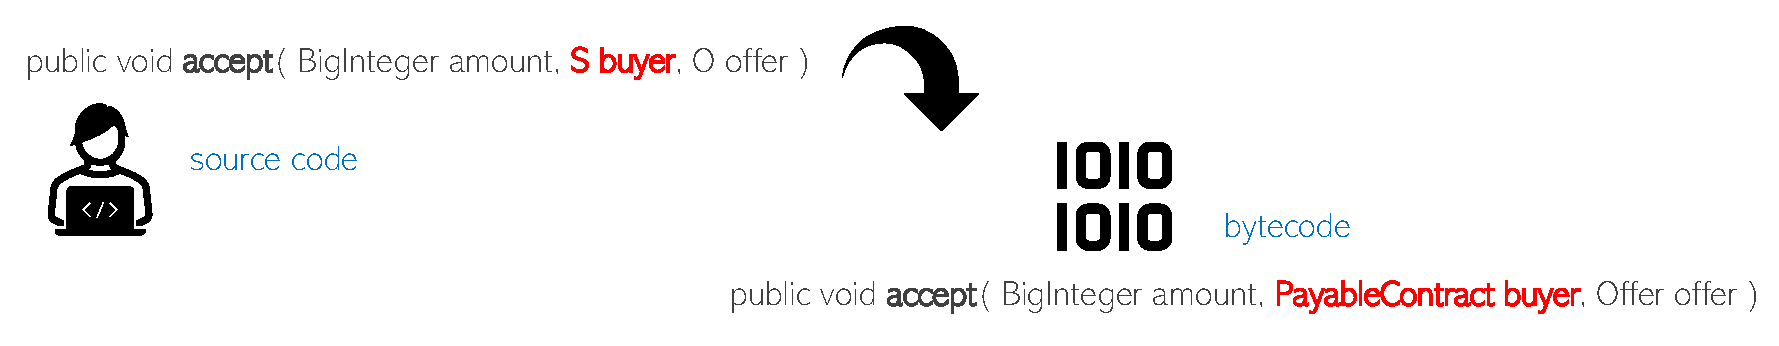
\includegraphics[width=0.8\linewidth]{figures/java_generics_erasure}
\caption{Example of generics implementation by erasure in Java.}
\label{figure.java_generics_erasure}
\end{figure*}

In order to understand the mechanism of erasure, consider for instance
the interface \<SharedEntity> in Fig.~\ref{fig:shared_entity} and its method \<accept>.
The functionality of \<SharedEntity> will be discussed later (Sec.~\ref{sec:shared_entities}).
Here, we only consider how its generic type parameters get compiled.
Namely, \<SharedEntity> uses two generic type parameters \<S> and \<O>, that must be provided
whenever a client creates a concrete implementation of the interface.
Such generic parameters have an upper bound: \<S> can only be a subtype of \<PayableContract>,
while \<O> can only be a subtype of {\codesize\texttt{Offer<S>}}. If we check the bytecode
generated for \<SharedEntity>, we will see that \<accept> is declared, in bytecode, as
\<void accept(BigInteger amount, PayableContract buyer, Offer offer)>, that is,
the two type variables \<S> and \<O> have been \emph{erased} and replaced with their
respective upper bound, as illustrated in Fig.\,\ref{figure.java_generics_erasure}.



Erasure weakens the type information of the compiled code. It is the responsibility of the
compiler to guarantee that types are still respected, in all implementations of \<SharedEntity>.
In Java, the compiler guarantees type correctness and the Java language remains strongly-typed,
also in the presence of generic types,
if no \emph{unchecked operations} are performed~\cite{NaftalinW06} (such as casts to generic types,
that are unchecked for a limitation of the Java bytecode).
However, this guarantee applies to Java source code compiled by the Java compiler,
not to bytecode that can be generated manually, in order to attack instances of
the \<SharedEntity> class, as we will show later.

\section{Shared Entities using Generics}\label{sec:shared_entities}

A \emph{shared entity} is a concept that often arises in blockchain
applications. Namely, a shared entity is something divided into \emph{shares}. Participants,
that hold shares, are called \emph{shareholders} and can dynamically
sell and buy shares. An example of a shared entity is a corporation,
where shares represent units of possess of the company. Another example is
a voting community, where shares represent the voting power of each given voter.
A further example is the set of the validator nodes of a proof of stake blockchain,
where shares represent their voting power and remuneration percentage.

\begin{figure}[ht]
  \begin{center}
    \begin{lstlisting}[language=Takamaka]
public interface SharedEntity
      <S extends PayableContract, O extends Offer<S>>
      extends SharedEntityView<S> {

  @View
  StorageSetView<O> getOffers();

  @View
  BigInteger sharesOnSaleOf(S shareholder);

  @FromContract(PayableContract.class) @Payable
  void place(BigInteger ticket, O offer);

  @FromContract(PayableContract.class) @Payable
  void accept(BigInteger ticket, S buyer, O offer);

  class Offer<S extends PayableContract> extends Storage {
    public final S seller;
    public final BigInteger sharesOnSale;
    public final BigInteger cost;
    public final long expiration;

    public Offer(S seller, BigInteger sharesOnSale, 
                 BigInteger cost,long duration) {
      this.seller = seller;
      this.sharesOnSale = sharesOnSale;
      this.cost = cost;
      this.expiration = now() + duration;
    }

    @View
    public boolean isOngoing() {
      return now() <= expiration;
    }
  }
}
    \end{lstlisting}
  \end{center}
  \caption{A simplified part of our shared entity interface.}\label{fig:shared_entity}
\end{figure}

In general, two concepts are specific to each implementation of shared entities:
who are the potential shareholders and how offers for selling shares work.
Therefore, one can parameterize the interface of a shared entity with two type variables:
\<S> is the type of the shareholders and \<O> is the type of the sale offers of shares.



\begin{figure}[tp]
  \begin{center}
    \begin{lstlisting}[language=Takamaka]
public class SimpleSharedEntity
    <S extends PayableContract,O extends Offer<S>>
    extends PayableContract implements SharedEntity<S,O> {

  private StorageTreeMap<S,BigInteger> shares = new StorageTreeMap<>();
  private StorageSet<O> offers = new StorageTreeSet<>();

  public SimpleSharedEntity
      (S shareholder, BigInteger share) {
    addShares(shareholder, share);
  }

  @Override @View
  public final BigInteger sharesOf(S shareholder) {
    return shares.getOrDefault(shareholder, ZERO);
  }

  @Override @FromContract(PayableContract.class) @Payable
  public void place(BigInteger amount, O offer) {
    require(offer.seller == caller(), "unauthorized");
    require(shares.containsKey(offer.seller), "unauthor.");
    require(sharesOf(offer.seller) - sharesOnSaleOf(offer.seller) >= 
            offer.sharesOnSale, "not enough shares");
    offers.add(offer);
  }

  @Override @FromContract(PayableContract.class) @Payable
  public void accept(BigInteger amount, S buyer, O offer) {
    require(caller() == buyer, "unauthorized");
    require(offers.contains(offer), "unknown offer");
    require(offer.isOngoing(), "the offer is not ongoing");
    require(offer.cost <= amount, "not enough money");
    offers.remove(offer);
    removeShares(offer.seller, offer.sharesOnSale);
    addShares(buyer, offer.sharesOnSale);
    offer.seller.receive(offer.cost);
  }

  @Override @View
  public final BigInteger sharesOnSaleOf(S shareholder) {
    return offers.stream()
     .filter(o -> o.seller == shareholder && o.isOngoing())
     .map(offer -> offer.sharesOnSale)
     .reduce(ZERO, BigInteger::add);
  }
}
    \end{lstlisting}
  \end{center}
  \caption{A simplified part of our implementation of the shared entity interface.}\label{fig:simple_shared_entity}
\end{figure}

The \<SharedEntityView> interface at the top of the hierarchy in Fig.~\ref{fig:hierarchy-entities}
defines the read-only operations on a shared entity. This view is \emph{static}, in the sense that it
does not specify the operations for transfers of shares. Therefore, its only type parameter is \<S>:
any contract can play the role of the type for the shareholders of the entity.
Method \<getShares> yields a snapshot of the
current shares of the entity (who owns how much). Method \<getShareholders> yields the shareholders.
It is not \<@View>, since it creates a new stream, which is a side-effect.
Method \<isShareholder> checks if an object is a shareholder. Method \<sharesOf> yields
the number of shares of a shareholder. As typical in Takamaka, a \<snapshot> method allows one
to create a frozen read-only copy of an entity (in constant time), useful when an entity must be queried from
a client without the risk of race conditions if another client is modifying the same entity concurrently.

The \<SharedEntity> subinterface adds methods for transfer of shares
(see Fig.~\ref{fig:shared_entity}).
It includes an inner class \<Offer> that models sale offers:
it specifies who is the seller of the shares,
how many shares are being sold, the requested price and the expiration of the offer.
Method \<isOngoing> checks if an offer has not expired yet.
Implementations can subclass \<Offer> if they need more specific offers.
Offers can be placed on sale
by calling the \<place> method with a sale \<offer>.
This method is annotated as \<@FromContract> since the caller must be
identified (or otherwise anybody could sell the shares of anybody else) and
as \<@Payable> so that implementations can require
to pay a \<ticket> to place shares on sale.
The sale offer is passed as a parameter to \<place>, hence it must have been created before calling that method.
The set of all sale offers is available through \<getOffers>. Method \<sharesOnSale> yields the
cumulative number of shares on sale for a given shareholder.
Who wants to buy shares calls method \<accept> with the accepted \<offer>
and with itself as \<buyer> (the reason will be explained soon)
and becomes a new shareholder or increases
its cumulative number of shares (if it was a shareholder already).
Also this method is \<@Payable>, since its caller must pay \<ticket> $\ge$ \<offer.cost>
coins to the seller.
This means that shareholders must be able to receive payments and that
is why \<S extends PayableContract>: only \<PayableContract>s are guaranteed to have a
\<receive> method in Takamaka.

\begin{figure}[ht]
\centering
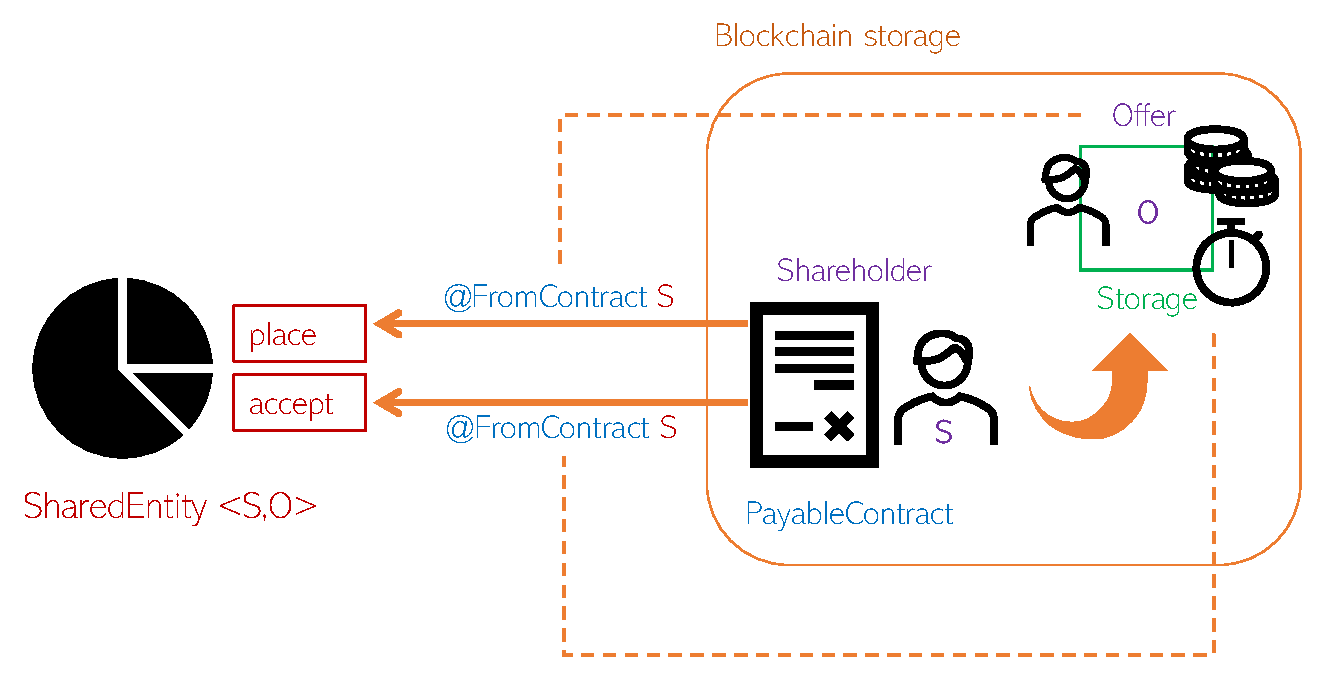
\includegraphics[width=.9\linewidth]{figures/shared_entity}
\caption{Exemplification of a Takamaka shared entity and of its connections with the objects persisted in the blockchain.}
\label{figure.shared_entity}
\end{figure}

As said before, the annotation \<@FromContract> on both \<place> and \<accept> enforces that only
contracts can call these methods.
These callers must be (old or new) shareholders,
hence they must have type \<S>. Therefore, one would like to write
\<@FromContract(S.class)>. Unfortunately, Java does not allow a generic type variable \<S>
in the syntax \<S.class>. Due to this syntactical limitation of Java,
the best we could write in Fig.~\ref{fig:shared_entity} is \<@FromContract(PayableContract.class)>,
which allows \emph{any} \<PayableContract> to call these methods, not just those of type \<S>.
Since the syntax of the language does not support our abstraction, we will have to
program explicit dynamic checks in code, as shown later, and this will be the reason of the
parameter \<buyer> in \<accept>.

Fig.~\ref{fig:simple_shared_entity} shows a portion of our \<SimpleSharedEntity>
implementation of the \<SharedEntity> interface in Fig.~\ref{fig:shared_entity}, that
uses two fields: \<shares> maps each shareholder to the amount of shares the it holds and
\<offers> collects the offers that have been placed.
The constructor initially populates the map \<shares> with the initial shareholder.
Other shareholders can be added later, by buying shares\footnote{In the real code, the class has
  constructors to create shared entities with a \emph{set} of initial shareholders. This paper
  reports a simplification of the actual code.}.
Method \<sharesOf> simply accesses
\<shares>, by using zero as default. Method \<place> requires its \<caller()> to be
the seller identified in the \<offer>. This forbids shareholders to sell shares on behalf of others.
Moreover, this guarantees that the caller has type \<S>, the type of \<offer.seller>.
As it has been said before, this cannot be expressed with the syntax of the language.
Method \<place> further requires the seller to be a shareholder with at least \<offer.sharesOnSale>
shares not yet placed on sale. This forbids to oversell more shares
than one owns. At the end, \<place> adds the \<offer> to the set of \<offers>.
Method \<accept> requires that who calls the method must be \<buyer>. Hence, successful
calls to \<accept> can only pass the same caller for \<buyer>. This is a trick to enforce the
caller to have type \<S>, since the syntax of the language does not allow one to express it,
as we explained before. Then \<accept> requires the \<offer> to exist, to be still ongoing
and to cost no more than the \<amount> of money provided to \<accept>. If that is the case,
the \<offer> is removed from the \<offers>, shares are moved from seller to buyer (code not
shown in Fig.~\ref{fig:simple_shared_entity}) and the seller of the \<offer>
receives the required price \<offer.cost>.

\section{An Attack to the Shared Entities Contract}\label{sec:attack}

This paper originated from an actual security issue that we found in our code
that used shared entities in order to model the validators of a blockchain.
Namely, the Hotmoka blockchain is built over Tendermint~\cite{Kwon14}, a
generic engine for replicating an application over a network of nodes. In our case,
the application is the executor of smart contracts in Java, such as that in
Fig.~\ref{fig:simple_shared_entity}. Tendermint is based on a proof of stake
consensus, which means that a selected dynamic subset of the nodes is in charge of
validating the transactions and voting their acceptance. Validator nodes are
represented by \<Validator> objects, that are externally owned accounts
with an extra identifier derived from their public key (see Fig.~\ref{fig:validator}).
This identifier is public information, reported in the blocks or easily eavesdropped.
At each block, the reward for the block is distributed to the validators.
Tendermint applications can implement their own
policy for changing the validator set dynamically. In our case, the validator set
and the distribution of the reward is implemented by a subclass
\<Validators> of \<SimpleSharedEntity> whose type \<S> for the shareholders
has been set to \<Validator>. Shares are voting power in this case.

\begin{figure}[t]
  \begin{center}
    \begin{lstlisting}[language=Takamaka]
public final class Validator extends ExternallyOwnedAccount {
  private final String id;

  public Validator(String publicKey) {
    super(publicKey);
    this.id = /* derived from publicKey as specified in Tendermint's spec */
  }

  public @View String id() {
    return id;
  }
}
    \end{lstlisting}
  \end{center}
  \caption{The representation of a validator of a Tendermint blockchain.
  Its full code is available at \url{https://github.com/Hotmoka/hotmoka/blob/master/io-takamaka-code/src/main/java/io/takamaka/code/governance/tendermint/TendermintED25519Validator.java}.}\label{fig:validator}
\end{figure}

Since shares of a \<SimpleSharedEntity> can be sold and bought, the set of validators
is dynamic. Users can sell or buy voting power in order to invest in the blockchain
and earn rewards. At each block creation, Hotmoka calls method \<getShareholders>
on the shared entity and informs the
underlying Tendermint engine about the identifiers of the validator nodes for the next blocks.
Tendermint expects such validators to mine and vote the subsequent blocks, until a change in the
validators set occurs.

It is important that the shareholders be instances of \<Validator>, since that class enforces the
match between their public key, that identifies who can use the reward sent to the validator,
and the Tendermint identifier of the validator, that identifies which node of the blockchain
must do the validation work (Fig.~\ref{fig:validator}).
If it were possible to add a shareholder of another
type \<Attacker>, the latter could declare the identifier of a node that does not correspond to its
public key (see Fig.~\ref{fig:attacker}):
the node (belonging to the \emph{victim}) would do the work while the owner
of the private key of the \<Attacker> could just wait and earn the reward.
A sort of validator's slavery.

\begin{figure}[t]
  \begin{center}
    \begin{lstlisting}[language=Takamaka]
public class Attacker extends ExternallyOwnedAccount {

  public Validator(String publicKey) {
    super(publicKey);
  }

  public @View String id() {
    return /* id of the victim node of the blockchain */
  }
}
    \end{lstlisting}
  \end{center}
  \caption{An attacker that exploits a blockchain node for validation and fraudolently earns the reward of its work.}\label{fig:attacker}
\end{figure}


\section{Fixing the Compilation of the Contract} \label{sec:fix}

The security issue in Sec.~\ref{sec:attack} is due to the
over-permissive erasure of the signature of method \<accept>,
where \<buyer> is given type \<PayableContract>.
Therefore, a solution is to oblige the compiler to generate a more
restrictive signature where, in particular, the parameter \<buyer>
has type \<TendermintED25519Validator>: only that type of accounts
must be accepted for the validators, consequently banning instances of \<Attacker>.

\begin{figure}[t]
  \begin{center}
    \begin{lstlisting}[language=Java]
public class TendermintValidators
    extends AbstractValidators<TendermintED25519Validator> {

  public TendermintValidators
        (TendermintED25519validator[] validators, 
         BigInteger[] powers) {
    super(validators, powers);
  }

  @Override @FromContract(PayableContract.class) @Payable
  public void accept
    (BigInteger amount, 
     TendermintED25519Validator buyer, 
     Offer<TendermintED25519Validator> offer) {
    super.accept(amount, buyer, offer);
  }
}
    \end{lstlisting}
  \end{center}
  \caption{The shared entity of the validators of a Hotmoka blockchain built over Tendermint.
  Its full code is available at \url{https://github.com/Hotmoka/hotmoka/blob/master/io-takamaka-code/src/main/java/io/takamaka/code/governance/tendermint/TendermintValidators.java}.}\label{fig:solution}
\end{figure}

The fixed code is shown in Fig.~\ref{fig:solution}. The only difference is that method
\<accept> has been redefined to enforce the correct type for \<buyer>. For the rest, that method
delegates to its implementation inherited from \<AbstractValidators>, through a call
to \<super.accept>.
It is important to investigate which is the Java bytecode generated from
the code in Fig.~\ref{fig:solution}. Since Java bytecode does not allow one to redefine a method
and modify its argument types, the compiled bytecode actually contains \emph{two}
\<accept> methods, as follows:

\begin{lstlisting}[language=JavaBytecode]
public class TendermintValidators extends AbstractValidators {
  ...
  
  public void accept
   (BigInteger,TendermintED25519Validator,Offer)
   aload_0
   aload_1
   aload_2
   aload_3
   invokespecial AbstractValidators
     .accept(BigInteger,PayableContract,Offer)
   return

  // synthetic bridge method
  public void accept(BigInteger,PayableContract,Offer)
   aload_0
   aload_1
   aload_2
   checkcast TendermintED25519Validator
   aload_3
   invokevirtual accept
      (BigInteger,TendermintED25519Validator,Offer)
   return
}
\end{lstlisting}

\noindent
The first \<accept> method above is the compilation of that from Fig.~\ref{fig:solution}:
it delegates to the \<accept> method of the superclass \<AbstractValidators>. The second
\<accept> method above is a \emph{bridge method} that the compiler generates in order to guarantee
that all calls to the erased signature \<accept(BigInteger,PayableContract,Offer)> actually
get forwarded to the first, redefined \<accept>. It casts its \<buyer> argument
into \<TendermintED25519Validator> and calls the first \<accept>. This
bridge method and its checked cast guarantee that only \<TendermintED25519Validator>s
can become validators. For instance, an instance of \<Attacker> (Fig.~\ref{fig:attacker})
cannot be passed to the first \<accept> (type mismatch) and makes the second \<accept>
fail with a class cast exception. The \emph{Consistency of Shareholders} holds
for instances of \<TendermintValidators> now and the attack in Sec.~\ref{sec:attack} cannot occur
anymore.

The solution of redefining method \<accept> can be seen as a limited form of heterogeneous
compilation of generics, restricted to a specific method and forced manually.
It is interesting to consider which methods
would need that redefinition, in general. They are those that have a parameter of a generic type
that is restricted in a subclass. For instance, method \<accept> in
Fig.~\ref{fig:shared_entity} has parameters \<buyer> and \<offer> of generic type
\<S> and \<O>, respectively. The subclass in Fig.~\ref{fig:abstract_validators} restricts
\<S> to be a \<TendermintED25519Validator> and \<O> to be
an {\codesize\texttt{Offer<TendermintED25519Validator>}}. Hence we must redefine
\<accept> in the subclass with the more specific types for the \<buyer> and \<offer>
parameters. In the future, a compiler might perform this automatically or a static analysis
tool might issue a warning when such redefinition is needed. Currently, however, this is
left to the programmer of the smart contracts, who might overlook the issue
and give rise to security issues, as shown in Sec.~\ref{sec:attack}.


\section{Related Work}\label{sec:related_work}

\todo{Forse questa parte va spostata.}


\textbf{Generics Compilation --} Generics is a way for writing code parametrized by type, in other words a same piece of code can be written by using a type placehorder (ie. parameter) and then instantiated it for a specific type arguments. There exists two common ways to implement generics in a programming language that are often described in literature\,\cite{generics_categories} as \textit{heterogeneous} and \textit{homogeneous}. In the heterogeneous approach the code is specialized for each instance of the generic parameter, this is the approach adopted by the C++ \emph{templates}. Conversely, the homogeneous approach is the one provided by Java or .Net, in this case only one instance of the code is maintained that is shared by all generic instances. This implementation is based on the type \emph{erasure} mechanism in which the generic parameter is replaced by the upwards bound of each instance, most often \<Object>.
%
Even if the heterogeneous approach is the most safe one, it is rarely applied in particular in resource-constrained applications, because in this case the code size  may dramatically increase as some code is duplicated \cite{generics_embedded_systems}. Conversely, the latter approach ensures a smaller consumption of resources but can lead to the problems described in this paper. \\

\noindent
\textbf{Smart contracts vulnerabilities --} It has been estimated that on average, software developers make 100 to 150 errors for every thousand lines \cite{software_engineering}.
In 2002, the National Institute of Standards and Technology (NIST) estimates that the economic costs of faulty software in the US is about tens of billions of dollars per year and represent approximately just under 1 percent of the nation's gross domestic product (GDP). The effects induced by errors in software development are even worse when such piece of software represents a smart contract for two main reasons. First of all, it is usually impossible to change a smart contract once it has been deployed, the immutability is one of its main characteristics and errors are treated as intended behaviours. Secondly, smart contracts often store and
manage critical information such as digital assets and identities. For these reason several analysis of smart contracts vulnerabilities have been performed and some static analysis tools have been developed.



\begin{itemize}
\item Solythesis \cite{solythesis_solidity_validation}: A compilation tool for smart contracts which provides an expressive language for specifying desired safety invariants. Given a smart contract and a set of user defined invariants, it is able to produce a new enriched contract which will reject all transactions that violate such invariants.

\item Another solutions which is based on bytecode rewriting is presented in \cite{bytecode_rewriting}, where the authors propose the enforcement of security polices through the enhancement of EVM bytecode. More specifically, the disassembled bytecode is instrumented through new security guard code that enforces the desired policy. Their initial efforts are mainly focused on the  verification of arithmetic operations, such as the prevention of overflows; while in the future they will focus on
adding the verification of memory access operations.

\item SafeVM \cite{safevm}:  A  verification tool for Ethereum smart contracts which directly works on EVM bytecode and exploits the state-of-the-art verification engines already available for C programs. The basic idea is to take as input a smart contract in compiled EVM\ bytecode which can eventually contain some \<assert> or \<require> annotations, then such bytecode is decompiled and converted into a C program with \<ERROR> annotations. This produced C program can be verified by using existing verification tools.
 
\item In \cite{hol_smart_constracts} the authors propose the use of the existing Isabelle/HOL tool with the specification of a formal logic for EVM bytecode, in order to provide a verification tool for Ethereum smart contracts. More specifically, the desired properties  of contracts are stated in a pre/postcondition style, while the verification is done by recursively structuring contracts as a set of basic blocks
down to the level of instructions.

\item Scilla \cite{scilla} is a new programming language for safe smart contracts which as been tailored taking   System F as a foundational calculus. It is able to provide strong safety guarantees by means of type soundness. Thanks to its minimalistic nature, it has been possible to define also a generic and extensible framework for lightweight verification of smart contracts by means of user-defined domain-specific analyse. \todo{Ci sono i generics oppure essendo un linguaggio minimale non si pongono il problema??}



 
\end{itemize}

Given the plurality of verification tools that have been developed for indentifying security bugs in smart contracts, a unified and standard approach for evaluating their accuracy and performances have been developed in \cite{effectiveness_analysis_tools}. This automated and systematic approach, called SolidiFI, consists in injecting bugs into all potential locations in a smart contract, in order to introduce different kinds of vulnerabilities, and then using several static analysis tools to identify which bugs each of them is able to detect.



\section{Conclusion}\label{sec:conclusion} 

This paper has shown that generic types can be useful in the definition
of smart contracts, but introduce risks of security since in many
programming languages, including Java, they get erased at compile time
into types that might be too permissive for low level calls, such as
those that start blockchain transactions. Note that using a programming
language without generics is not the solution: Solidity has no generics
and consequently erases \emph{all} reference types into \<address>.
That is the worst possible erasure.

The solution in this paper has been to redefine a method with an argument
of generic type in such a way to call its superclass
(see \<accept> in Fig.~\ref{fig:solution}). This fixes the security risk,
but cannot be regarded as an elegant solution. It is just a trick that
works because it forces the compiler to generate some kind of bytecode.
A \emph{smarter} compiler might recognize the redefined \<accept> as
\emph{useless} and just remove it. This would recreate the issue that
we have just solved. That is, our solution works only for the way
compilers compile \emph{today}.

With hindsight, it is questionable to have implemented generics by erasure
and code instrumentation (bridge methods). If generics would be present
and checked at bytecode level, the attack in Sec.~\ref{sec:attack} would just
be impossible. Currently, generics can only exist as bytecode annotations,
but they are not mandatory and are not used by the Java virtual machine
that runs the bytecode. The same consideration might be applied beyond
generics: many features of modern programming
languages have no direct low-level
counterpart but are implemented via instrumentation, starting from
inner classes and closures. This is fine at source level, but allows
low-level calls to easily circumvent
the encapsulation guarantees of the language. When immerged in a permissionless
blockchain, such features become dangerous attack surfaces.


%% -----------------------------------------------------------------------------

% \begin{appendices}

% \section{Section title of first appendix}\label{secA1}

% An appendix contains supplementary information that is not an essential 
% part of the text itself but which may be helpful in providing a more
% comprehensive understanding of the research problem or it is information 
% that is too cumbersome to be included in the body of the paper.

%%==============================================%%
%% For submissions to Nature Portfolio Journals %%
%% please use the heading ``Extended Data''.    %%
%%==============================================%%

%%=============================================================%%
%% Sample for another appendix section                         %%
%%=============================================================%%

%% \section{Example of another appendix section}\label{secA2}%
%% Appendices may be used for helpful, supporting or essential material that would otherwise 
%% clutter, break up or be distracting to the text. Appendices can consist of sections, figures, 
%% tables and equations etc.

%\end{appendices}

%%===========================================================================================%%
%% If you are submitting to one of the Nature Portfolio journals, using the eJP submission   %%
%% system, please include the references within the manuscript file itself. You may do this  %%
%% by copying the reference list from your .bbl file, paste it into the main manuscript .tex %%
%% file, and delete the associated \verb+\bibliography+ commands.                            %%
%%===========================================================================================%%

\bibliographystyle{elsarticle-num}
\bibliography{biblio}% common bib file
%% if required, the content of .bbl file can be included here once bbl is generated
%%\input sn-article.bbl

%% Default %%
%%\input sn-sample-bib.tex%

\end{document}
